\documentclass[11pt]{article}
% --- Encoding e font ---
\usepackage[utf8]{inputenc}
\usepackage[T1]{fontenc}
\usepackage{lmodern}

% --- Matematica ---
\usepackage{amsmath,amssymb,amsfonts,gensymb,amsthm}
\DeclareMathOperator*{\argmin}{arg\,min}
\DeclareMathOperator*{\argmax}{arg\,max}
\usepackage{centernot}
% --- Grafica, colori, float ---
\usepackage{graphicx}
\usepackage[dvipsnames]{xcolor}
\usepackage{float}
% --- Liste e ambienti ---
\usepackage{enumitem}
% --- Caption, numerazione figure ---
\usepackage{caption}
\usepackage{chngcntr}
% --- Caption, numerazione figure ---
\captionsetup{font=small, labelfont=bf, textfont=it}
% --- Indice/TOC personalizzazione (se ti serve) ---
\usepackage{tocloft}
% --- colorbox
\usepackage[most]{tcolorbox}
%--- spazio tra le riga
\usepackage{parskip}
\setlength{\parskip}{0.15cm}
% Elenchi compatti:
\setlist[itemize]{ topsep=2pt, itemsep=0pt, parsep=0pt}
\setlist[enumerate]{topsep=2pt, itemsep=0pt, parsep=0pt}

% Per il codice
\usepackage{listings}
% Definisci i colori esatti di VS Code (tema Light+)
\definecolor{vscodeblue}{RGB}{0,0,255}          % Keywords
\definecolor{vscodeorange}{RGB}{163,21,21}      % Strings
\definecolor{vscodegreen}{RGB}{0,128,0}         % Comments
\definecolor{vscodepurple}{RGB}{197,134,192}    % Control flow e import
\definecolor{vscodeyellow}{RGB}{121,94,38}      % Functions
\definecolor{vscodebg}{RGB}{255,255,255}        % Background
\definecolor{vscodeframe}{RGB}{200,200,200}     % Frame

% Configurazione Python stile VS Code
\lstdefinestyle{vscode}{
    language=Python,
    alsoletter={.},
    backgroundcolor=\color{vscodebg},
    commentstyle=\color{vscodegreen}\itshape,
    numberstyle=\tiny\color{gray},
    stringstyle=\color{vscodeorange},
    basicstyle=\ttfamily\small,
    breakatwhitespace=false,
    breaklines=true,
    captionpos=b,
    keepspaces=true,
    numbers=left,
    numbersep=8pt,
    showspaces=false,
    showstringspaces=false,
    showtabs=false,
    tabsize=4,
    frame=single,
    rulecolor=\color{vscodeframe},
    framesep=10pt,
    xleftmargin=15pt,
    framexleftmargin=15pt,
    % Resetta tutte le keyword e ridefiniscile
    morekeywords={},
    deletekeywords={for,if,while,else,elif,return,break,continue,try,except,finally,with,as,pass,raise,assert,import,from},
    % Keywords blu
    keywordstyle=\color{vscodeblue}\bfseries,
    morekeywords={def,class,lambda,and,or,not,is,in,del,global,nonlocal,yield,await,async,True,False,None,self},
    % Control flow VIOLA
    keywordstyle=[2]\color{vscodepurple}\bfseries,
    morekeywords=[2]{for,if,while,else,elif,return,break,continue,try,except,finally,with,as,pass,raise,assert,import,from},
    % Funzioni
    emph={sqrt,print,input,range,len,str,int,float,list,dict,set,tuple},
    emphstyle=\color{vscodeyellow}
}
\lstset{style=vscode}

%-- for definition (POI definisci defbox)
\newtcolorbox{defbox}[1]{
    colback=gray!10,
    colframe=gray!50,
    fonttitle=\bfseries,
    coltitle=black,
    title=\mbox{#1},  % Cambiato qui
    sharp corners,
    boxrule=0.5pt, breakable}
%-----
%-----
\usepackage{needspace}
%---- Notebox definition \begin{noteboxtitle}{title}
\newtcolorbox{noteboxtitle}[1]{
    colback=white,
    colframe=black!90,
    boxrule=0.8pt,
    arc=3mm,
    title=#1,
    fonttitle=\bfseries,
    left=5pt,
    right=5pt,
    top=5pt,
    bottom=5pt,
      breakable
}

% --- comment
\usepackage{comment}
% --- Margini ---
\usepackage[a4paper,
    top=2.5cm,
    bottom=2.5cm,
    left=2.5cm,
    right=2.5cm,
    bindingoffset=0.5cm
]{geometry}
% --- Titolo con immagine (opzionale) ---
\usepackage{titlepic} % solo se usi \titlepic
% --- Hyperref VA QUASI SEMPRE PER ULTIMO ---
\usepackage{hyperref}
\usepackage{adjustbox}
\usepackage{xltabular}
\usepackage{booktabs}
\raggedbottom


%---Per spezzare le tabelle
\usepackage{longtable}


% --- New structure for Example
\newtheoremstyle{smallexample}
  {3pt}% Space above
  {3pt}% Space below
  {\small}% Body font - testo dell'esempio piccolo
  {}% Indent amount
  {\small\bfseries}% Theorem head font - "Example 18.1" piccolo e grassetto
  {.}% Punctuation after theorem head
  {.5em}% Space after theorem head
  {}% Theorem head spec
\theoremstyle{smallexample}
\newtheorem{example}{Example}[section]
\usepackage[version=4]{mhchem}
\graphicspath{{Images/}}

 %% --- Definizione prima pagina 


%%___NEW COMMAND
\newcommand{\vs}{\vspace{0.2\baselineskip}}



%%%--- Librerie per grafici

\usepackage{tikz}
\usetikzlibrary{positioning, arrows.meta, shapes.geometric, calc}
\usepackage{tcolorbox}
\tcbuselibrary{breakable, skins}



\parindent 0px
\title{\Huge Data Mining and Machine Learning}
\author{\Large Gennaro Basile}
\date{\today}

\titlepic{
    \begin{center}
        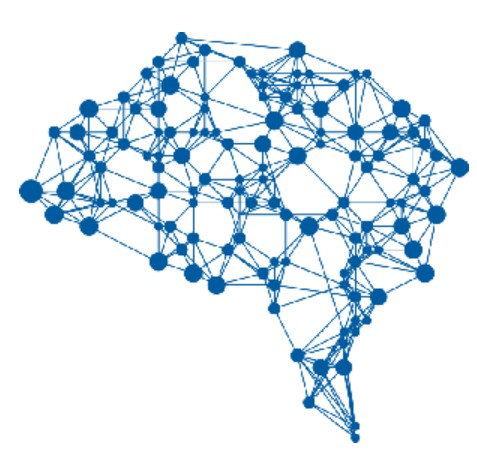
\includegraphics[scale=1]{0.DeepLearningLogo.jpg}
    \end{center}}



\begin{document}
\maketitle
\counterwithin{figure}{subsection}
\captionsetup[figure]{labelfont=bf}

\pagebreak

%% -- Sommario
\tableofcontents
\pagebreak



\section{Introduction to Data Mining}

\subsection{What is Data Mining?}

\begin{defbox}{Data Mining}
    Data Mining is the process of extracting actionable insights and patterns from large batches of raw data, drawing from statistics, machine learning, and database systems.
\end{defbox}

The field is built on three pillars:
\begin{itemize}
    \item \textbf{Study}: Integrates ML, stats, and data engineering.
    \item \textbf{Raw Data}: Data requires collecting, cleaning, and formatting before use.
    \item \textbf{Insights}: The ultimate output is actionable knowledge, not just computation.
\end{itemize}

\subsection{Data and Data Sources}

Data is everywhere. Every real-world data mining project starts with identifying
\textbf{what data exists} and \textbf{where it comes from}. Raw data is a row vector
(or record) of values corresponding to measurements of all variables on one unit.

Main data sources include:
\begin{itemize}
    \item \textbf{Surveys}: standard structured data collected directly from respondents,
    organized into a units $\times$ variables matrix.
    \item \textbf{Sensors / IoT devices}: generate \textit{data streams}, i.e., sequences
    of digitally encoded coherent signals organized into packets.
    \item \textbf{Satellites}: collect image and spatial data via cameras.
    \item \textbf{Social Networks}: provide text data, image data, and graph data.
    \item \textbf{ECG sensors}: extract electrical heart signals representable as
    time series, together with standard patient demographic data.
    \item \textbf{Geographic maps}: provide spatial data.
\end{itemize}

\vs
Non-standard data types (images, audio, graphs) can always be transformed into
standard tabular format during pre-processing via a step called \textbf{featurization}.

\subsubsection{Raw Data and the Design Matrix}

\begin{defbox}{Design Matrix}
    A \textbf{Raw Data Set} or \textbf{Design Matrix} $\mathcal{D} = \{\mathbf{d}_n\}_{n=1}^{N}$
    is a collection of $N$ records, each being a $D$-dimensional row vector, measuring
    $D$ variables (features) on $N$ units (objects):
    \[
        \mathcal{D} \in \mathbb{R}^{N \times D}, \qquad
        \mathbf{d}_n = (x_n^1, x_n^2, \ldots, x_n^D) \in \mathbb{R}^D
    \]
    \begin{itemize}
        \item $N$ = \textbf{size} (number of records/units)
        \item $D$ = \textbf{dimensionality} (number of variables/features)
        \item Variables can be measured on \textbf{numerical}, \textbf{ordinal}, or
        \textbf{nominal} scale.
    \end{itemize}
\end{defbox}

Two important shapes of $\mathcal{D}$:
\begin{itemize}
    \item \textbf{Tall and skinny} ($N \gg D$): classic \textit{Big Data} scenario, many
    observations, few features. Example: click logs.
    \item \textbf{Short and fat} ($D \gg N$): \textit{Wide Data} scenario, few observations,
    many features. Example: genomics, where $D$ = number of genes $\sim 20{,}000$
    and $N$ = number of patients $\sim 100$.
\end{itemize}

When inputs are of \textit{variable size}, data is not
naturally a matrix. In these cases \textbf{featurization} converts each object
into a fixed-length vector, implicitly creating $\mathcal{D}$.

\vs

\begin{example}{\textbf{Building a Design Matrix}}

    Suppose we survey $N = 4$ students on $D = 3$ variables: age (numerical),
    grade (ordinal: 1--5), and major (nominal: CS=1, Stats=2).
    \[
        \mathcal{D} =
        \begin{pmatrix}
            22 & 4 & 1 \\
            24 & 3 & 2 \\
            21 & 5 & 1 \\
            23 & 2 & 2
        \end{pmatrix}
        \in \mathbb{R}^{4 \times 3}
    \]
    \begin{itemize}
        \item \texttt{Step 1}: $N = 4$ (rows = students), $D = 3$ (columns = features).

        \item \texttt{Step 2}: Row profile of student 1:
        $\mathbf{d}_1 = (22, 4, 1)$, a 3-dimensional vector.

        
        \item \texttt{Step 3}: Column profile of feature ``age'':
        $(22, 24, 21, 23)^T$: unidimensional distribution of one variable
        across all $N$ units.

        \item \texttt{Step 4}: Shape check: $N = 4 \approx D = 3$, neither tall-skinny
        nor short-fat; a balanced small dataset.
    \end{itemize}
\end{example}

\subsection{The Basic Data Types}

\subsubsection{Nondependency-oriented vs Dependency-oriented Data}

The fundamental distinction in data relies on whether records or features influence each other.

\begin{itemize}
    \item \textbf{Nondependency-Oriented}: Records are independent and identically distributed (i.i.d.). E.g., individual user profiles in an app.
    \item \textbf{Dependency-Oriented}: Implicit or explicit relationships exist. Ignoring them destroys information. E.g., time-series data or social graphs.
\end{itemize}

\subsubsection{Binary Data}

Binary data is a special case appearing in two contexts:

\begin{defbox}{Binary Data}
    \begin{itemize}
    \item \textbf{As categorical data}: each variable takes on one of at most two discrete
    values (e.g., yes/no, 0/1). 
    \item \textbf{As quantitative data}: an ordering exists between the two values.
    \begin{itemize}[label=$\cdot$]
    \item  \textbf{Setwise representation}: given a universe of items $\mathcal{I}$, a
    \textit{set element indicator} for set $S$ is:
    \[
        \mathbf{1}_S(e) =
        \begin{cases}
            1 & \text{if } e \in S \\
            0 & \text{otherwise}
        \end{cases}
    \]
    \end{itemize}
    \end{itemize}
\end{defbox}

Binary data is central to \textbf{market basket analysis}: each transaction is
encoded as a binary vector over all $d$ products.

\vs
\begin{example}{\textbf{Binary Encoding of Market Baskets}}

    Universe of items: $\mathcal{I} = \{$milk, bread, eggs, butter, juice$\}$,
    so $d = 5$.
    \begin{itemize}
        \item \texttt{Step 1}: Customer A buys $\{$milk, bread, butter$\}$.
        Binary encoding: $\mathbf{x}_A = (1, 1, 0, 1, 0)$.

        \item \texttt{Step 2}: Customer B buys $\{$bread, eggs, juice$\}$.
        Binary encoding: $\mathbf{x}_B = (0, 1, 1, 0, 1)$.

     
        \item \texttt{Step 3}: Construct the binary design matrix:
        \[
            \mathcal{D} =
            \begin{pmatrix}
                1 & 1 & 0 & 1 & 0 \\
                0 & 1 & 1 & 0 & 1
            \end{pmatrix}
            \in \{0,1\}^{2 \times 5}
        \]

   
        \item \texttt{Step 4}: The column \textit{bread} sums to 2 out of 2 transactions
        $\Rightarrow$ support of bread = 1.0.
    \end{itemize}
\end{example}


\subsubsection{Text Data}

Text is a classic example of \textbf{dependency-oriented} data: a document is a
string, and words depend on context and order.

\begin{defbox}{Text Data and the Document-Term Matrix}
    A text document corresponds to a \textbf{string}: a sequence of characters or
    words. Text is converted into a \textbf{vector-space representation} where each
    document becomes a $d$-dimensional vector of word frequencies (term frequencies).
    The result is a \textbf{document-term matrix} of size $n \times d$:
    \[
        \mathcal{D}_{\text{text}} \in \mathbb{R}^{n \times d}, \quad
        d_{ij} = \text{frequency of term } j \text{ in document } i
    \]

\end{defbox}

    This process is studied in \textbf{Natural Language Processing (NLP)}.
    A key challenge is \textbf{data sparsity}: most entries are zero because each
    document uses only a small fraction of the full vocabulary.

\vs
\begin{example}{\textbf{Building a Document-Term Matrix}}

    Vocabulary: $\mathcal{V} = \{$data, mining, learning, statistics$\}$, $d = 4$. \\
    Two documents:
    \begin{itemize}
        \item \texttt{Step 1 -- Documents}:
        \begin{itemize}
            \item $\text{Doc}_1$: ``data mining and data analysis''
            \item $\text{Doc}_2$: ``machine learning and statistics''
        \end{itemize}

        \vspace{0.2cm}
        \item \texttt{Step 2 -- Count frequencies}:
        \[
            \begin{array}{l|cccc}
                        & \text{data} & \text{mining} & \text{learning}
                        & \text{statistics} \\ \hline
                \text{Doc}_1 & 2 & 1 & 0 & 0 \\
                \text{Doc}_2 & 0 & 0 & 1 & 1
            \end{array}
        \]

        \vspace{0.2cm}
        \item \texttt{Step 3 -- Matrix}:
        $\mathcal{D}_{\text{text}} = \begin{pmatrix} 2 & 1 & 0 & 0 \\ 0 & 0 & 1 & 1
        \end{pmatrix} \in \mathbb{R}^{2 \times 4}$.


    \end{itemize}
\end{example}


\subsubsection{Dependency Oriented Data}

\begin{itemize}
    \item \textbf{Implicit Dependencies}
    Dependencies that are \textbf{not encoded} in the data structure but are known
    to typically exist due to the nature of the data generating process. A sensor
    reading at time $t$ is expected to be close to the reading at time $t+1$: a
    sudden large jump is unusual and potentially interesting for data mining.

\vspace{0.3cm}
\item \textbf{Explicit Dependencies}
    Dependencies that are \textbf{directly encoded} in the data via structural
    elements such as edges in a graph. Example: in a social network, an edge
    $(i, j)$ explicitly states that users $i$ and $j$ are friends.
\end{itemize}


\subsubsection{Time-Series Data}

Dependency-oriented data often hinges on time or sequence. 

\begin{defbox}{Time-Series Data}
    A \textbf{time series} contains values generated by \textbf{continuous measurements
    over time}. It is characterized by two types of attributes:
    \begin{itemize}
        \item \textbf{Contextual attributes}: define the context of the dependency,
        e.g., the timestamp $t_i$ of a sensor reading (unix time, unix microtime).
        \pagebreak

        \item \textbf{Behavioral attributes}: the values measured in a given context,
        e.g., temperature or pressure at time $t_i$.
    \end{itemize}
    When multiple sensors record synchronized readings, we obtain a
    \textbf{multidimensional time series}.
\end{defbox}






    \begin{itemize}
        \item \textbf{Time-Series}: Behavioral attributes are continuous/numeric. 
        \item \textbf{Discrete Sequence}: Behavioral attributes are categorical. The univariate case is a \textbf{string}.
    \end{itemize}



\subsubsection{Spatial Data and Trajectories}

Spatial data uses coordinates (Latitude, Longitude) as contextual attributes. When you combine spatial and temporal contexts, you get \textbf{spatiotemporal data}.



         \begin{figure}[H] 
        \centering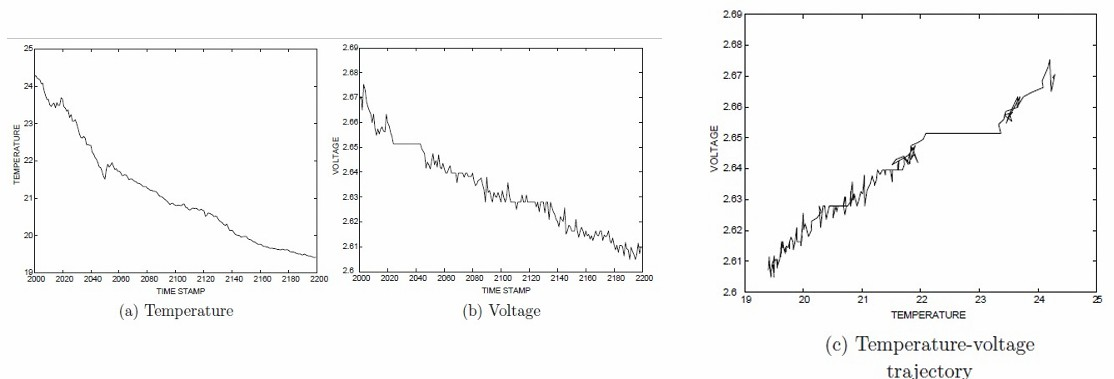
\includegraphics[scale=0.65]{1.Dependency Oriented Data.jpg}
        \caption{Dependency Oriented Data}
    \captionsetup{font=footnotesize}
    \end{figure}

\subsubsection{Network and Graph Data}

\begin{defbox}{Network / Graph Data}
    A network $G = (N, A)$ consists of a set of \textbf{nodes} $N$ (entities) and a set of \textbf{edges} $A$ (relationships). Edges encode \textbf{explicit dependencies} and can be directed (e.g., web links) or undirected.
\end{defbox}


\subsection{Data Preprocessing}

\subsubsection{The Data Preprocessing Pipeline}

Raw data is rarely ready for immediate analysis. It must pass through a structured \textbf{preprocessing pipeline} to become a clean, mathematical representation. This process consists of four sequential stages, accompanied by feedback loops:


    \begin{enumerate}
        \item \textbf{Data Collection}: Collecting raw data from sensors, databases, or APIs.
        \item \textbf{Feature Extraction}: Converting unstructured signals (logs, text, images) into structured, measurable features.
        \item \textbf{Data Cleaning \& Integration}: Handling missing/erroneous values and joining heterogeneous data sources (e.g., merging SQL tables).
        \item \textbf{Analytical Processing}: Applying machine learning algorithms (clustering, classification) to extract insights.
    \end{enumerate}
    \textbf{Feedback Loops}: If the analytical output is poor, the pipeline loops back to either re-extract features (e.g., tuning hyperparameters) or collect entirely new data.


         \begin{figure}[H] 
        \centering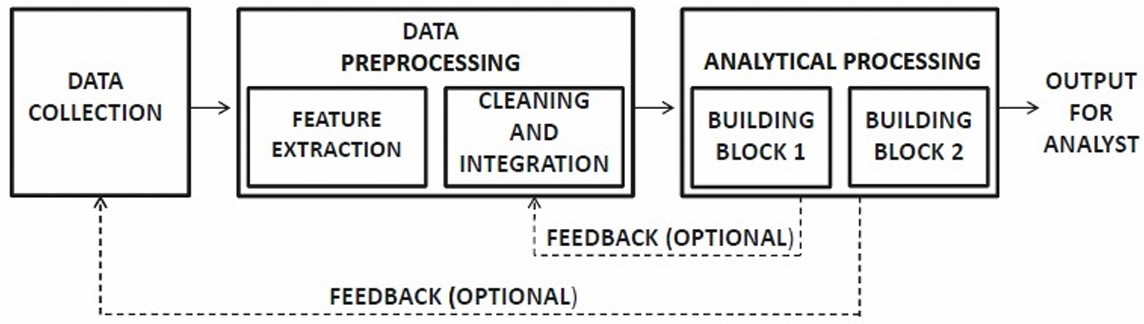
\includegraphics[scale=0.65]{2.Data Preprocessing Pipeline.jpg}
        \caption{Data Preprocessing Pipeline}
    \captionsetup{font=footnotesize}
    \end{figure}



In a corporate environment, Data Science does not exist in a vacuum; it drives \textbf{Business Intelligence}. Companies generate massive amounts of operational data. Data mining extracts hidden patterns from this data to support strategic decision-making and optimize resource allocation.



\subsubsection{The Retail Scenario: Merging Data Streams}

A classic Data Science problem involves combining disparate data types to create a unified \textbf{Design Matrix} ($\mathcal{D}$).

\begin{itemize}
    \item \textbf{Unstructured Web Logs}: Implicit, dependency-oriented behavior (e.g., timestamps, HTTP requests, clicks).
    \item \textbf{Structured Demographics}: Explicit, tabular data (e.g., age, income bracket).
\end{itemize}

By featurizing the web logs into a binary vector (e.g., $1$ if the user visited a product page, $0$ otherwise) and joining it with the demographic data on a common \texttt{CustomerID}, we create a unified dataset ready for clustering or recommendation algorithms.

\subsubsection{The Preprocessing Phase: The Real Bottleneck}

Preprocessing is universally acknowledged as the most time-consuming phase of any Data Science project. Advanced models cannot compensate for poor data quality. The phase breaks down into:

\begin{itemize}
    \item \textbf{Feature Extraction}: Deciding \textit{what} information to represent.
    \item \textbf{Data Cleaning}: Resolving \textit{erroneous values} (impossible data), \textit{missing values} (requiring imputation or row dropping), and \textit{inconsistent values} (logical contradictions).
    \item \textbf{Feature Transformation}: Rescaling data so no single feature dominates distance calculations. A standard approach is \textbf{Z-score normalization}: $\tilde{x} = \frac{x - \mu}{\sigma}$.
\end{itemize}

\subsubsection{Feature Subset Selection (FSS)}

Real-world datasets often suffer from the \textbf{Curse of Dimensionality} ($D$ is too large), making distances between data points uniform and algorithms ineffective. \textbf{FSS} identifies and retains only the most relevant subset of features, discarding the noise.

\begin{defbox}{FSS Paradigms}
    \begin{itemize}
        \item \textbf{Unsupervised Selection}: Evaluates features based on how well they form natural clusters (e.g., maximizing silhouette scores without knowing the target labels).
        \item \textbf{Supervised Selection}: Evaluates features based on their correlation with a known target label $y$ to maximize classification accuracy.
    \end{itemize}
\end{defbox}

\pagebreak

Common supervised techniques include:
\begin{itemize}
    \item \textbf{Filter methods}: Fast, statistical ranking (e.g., correlation matrices) independent of the ML model.
    \item \textbf{Wrapper methods}: Iteratively training a model on different feature subsets to find the best performer (computationally heavy).
    \item \textbf{Embedded methods}: Feature selection occurs naturally during model training (e.g., LASSO regression shrinking irrelevant feature weights to exactly $0$).
\end{itemize}



\subsection{The Major Building Blocks}

\subsubsection{Introduction}

Once data has been collected, preprocessed, and organized into a design matrix
$\mathcal{D} \in \mathbb{R}^{n \times d}$, the actual analytical work begins.
The \textbf{Major Building Blocks} are the four fundamental analytical tasks
that constitute the core of data mining. Every real-world data mining application
can be decomposed into one or more of these blocks:

\begin{itemize}
    \item \textbf{Association Pattern Mining}: Discovering relationships between \textit{columns} (features).
    \item \textbf{Data Clustering}: Discovering relationships between \textit{rows} (records).
    \item \textbf{Outlier Detection}: Identifying anomalous \textit{rows}.
    \item \textbf{Data Classification}: Predicting a specific \textit{column} (class label) based on the others.
\end{itemize}



\begin{defbox}{The Data Matrix}
    A multidimensional dataset is defined mathematically as a matrix:
    \[
        \mathcal{D} \in \mathbb{R}^{n \times d}
    \]
    where $n$ is the number of records (rows) and $d$ is the number of features (columns).
    \begin{itemize}
        \item \textbf{Row Profile} ($\mathbf{d}_i \in \mathbb{R}^d$): The complete measurement vector for a single unit. 
        \item \textbf{Column Profile} ($\in \mathbb{R}^n$): The distribution of a single feature across all units.
    \end{itemize}
\end{defbox}

         \begin{figure}[H] 
        \centering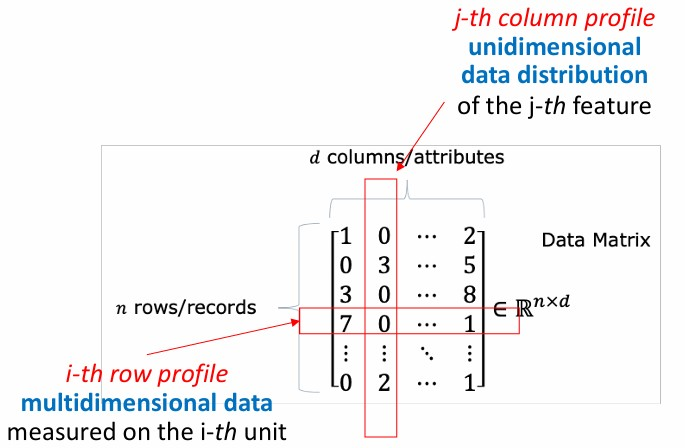
\includegraphics[scale=0.65]{3.Data Matrix.jpg}
        \caption{Multidimensional Data Set}
    \captionsetup{font=footnotesize}
    \end{figure}

The analytical building block you choose depends Depending on \textit{which
dimension} we analyze, we obtain different building blocks:

\begin{itemize}
    \item \textbf{Relationships between columns}
    \begin{itemize}
        \item \textit{Association Pattern Mining} (unsupervised): which columns
        tend to co-occur?
        \item \textit{Data Classification} (supervised): how do the other columns
        relate to one special column (the class label)?
    \end{itemize}
    \item \textbf{Relationships between rows}
    \begin{itemize}
        \item \textit{Clustering}: which rows are similar to each other?
        \item \textit{Outlier Analysis}: which rows are very different from all
        others?
    \end{itemize}
\end{itemize}

\subsubsection{Association Pattern Mining}

This operates primarily on \textbf{sparse binary databases} to find subsets of columns that frequently co-occur (e.g., market basket analysis).

\begin{defbox}{Association Rules}
    An association rule $A \Rightarrow B$ means \textit{if itemset $A$ appears, itemset $B$ also appears.} It is evaluated using two metrics:
    \begin{itemize}
        \item \textbf{Support ($s$)}: The fraction of total rows containing \textit{both} $A$ and $B$. ($\text{support}(A \cup B) \geq s$)
        \item \textbf{Confidence ($c$)}: The conditional probability that $B$ appears given $A$ appears. 
        \[ \text{confidence}(A \Rightarrow B) = \frac{\text{support}(A \cup B)}{\text{support}(A)} \geq c \]
    \end{itemize}
\end{defbox}

\vs

\begin{example}{\textbf{Support vs. Confidence in Retail}}

    If $A$ is ``Bread'' and $B$ is ``Butter'':
    \begin{itemize}
        \item Support tells you how important the rule is globally (e.g., 20\% of all transactions contain both).
        \item Confidence tells you how reliable the rule is locally (e.g., 90\% of people who buy bread will also buy butter).
    \end{itemize}
\end{example}

\subsubsection{Data Clustering}

Clustering is an \textbf{unsupervised} task that analyzes row relationships. The goal is to partition records into $k$ sets ($\mathcal{C}_1 \ldots \mathcal{C}_k$) so that intra-cluster similarity is high and inter-cluster similarity is low.

\begin{defbox}{Core Challenges of Clustering}
    Designing a clustering pipeline requires answering:
    \begin{itemize}
        \item \textbf{Distance Metric}: Euclidean for continuous data, Cosine/Jaccard for text or binary data.
        \item \textbf{Number of Clusters ($k$)}: Usually unknown; requires estimation techniques like the Elbow Method or Silhouette Scores.
        \item \textbf{Membership}: Hard clustering (each row belongs to exactly one cluster) vs. Soft clustering (rows have probability distributions across clusters).
    \end{itemize}
\end{defbox}

\vs
\textbf{Relevant applications of clustering:}
\begin{itemize}
    \item \textbf{Customer Segmentation} (Marketing): partition customers into
    homogeneous groups to target marketing campaigns.
    \item \textbf{Data Summarization}: identify $k$ representative points
    (centroids or medoids) that compactly describe the dataset.
    \item \textbf{Support for Outlier Analysis}: outliers are records that do
    not fit well into any cluster, and can be identified as those with high
    distance from their cluster center.
\end{itemize}

\subsubsection{Outlier Detection}

\begin{defbox}{Outlier Detection}
    Identifying rows in $\mathcal{D}$ that deviate so significantly from the norm that they appear to be generated by a \textbf{different underlying mechanism}.
\end{defbox}

\textbf{Crucial Data Science Insight}: Outliers are \textit{not} just bad data or garbage to be deleted. While they can be recording errors, they are often the most valuable data points in your matrix. 

\vs
\textbf{Applications:}
\begin{itemize}
    \item \textbf{Intrusion-detection systems}: network packets deviating from
    normal traffic patterns signal a possible attack.
    \item \textbf{Credit card fraud}: transactions whose amount, location, or
    time deviate from a customer's historical profile.
    \item \textbf{Interesting sensor events}: sudden spike in a sensor reading
    that may indicate equipment failure.
    \item \textbf{Earth science}: anomalous temperature or pressure readings that
    may indicate a geological event.
    \item \textbf{Medical diagnosis}: lab values far outside normal ranges for a
    patient's profile.
    \item \textbf{Law enforcement}: unusual financial transactions that may
    indicate money laundering.
\end{itemize}

\subsubsection{Data Classification}

Classification is the \textbf{supervised} counterpart to clustering. It requires a known \textbf{class label} ($y$) for a subset of the data. 

\begin{defbox}{Data Classification Workflow}
    Given a training matrix where each row is paired with a known label $y_i \in \{1 \ldots k\}$, the goal is to map features to labels by learning a model $\mathcal{M}$. This model is then used to predict the label of a new, unseen record $\overline{Y} \notin \mathcal{D}$.
\end{defbox}


The classification workflow involves two datasets:
\begin{itemize}
    \item \textbf{Training data}: records for which the class label $y_i \in
    \{1, \ldots, k\}$ is \textit{known}. Used to fit model $\mathcal{M}$.
    \item \textbf{Testing data}: records for which the class label is
    \textit{missing}. The trained model $\mathcal{M}$ predicts it.
\end{itemize}

\vs
\textbf{Applications of Data Classification:}
\begin{itemize}
    \item \textbf{Target marketing}: predict buying behaviors
    (e.g., will a customer buy product $X$? $\Rightarrow y \in \{0,1\}$).
    \item \textbf{Intrusion detection}: predict the possibility of a network
    intrusion from traffic features.
    \item \textbf{Supervised anomaly detection}: identify records belonging to
    a rare class (e.g., fraudulent transactions).
\end{itemize}

\vs
\begin{example}{\textbf{Classification vs. Clustering}}

    If you have a dataset of students with features $(x^1, x^2)$ representing (exam score, study hours):
    \begin{itemize}
        \item \textbf{Clustering} (Unsupervised): Running $k$-means ($k=2$) might naturally group the data into \textit{high performers} and \textit{low performers} based purely on spatial distance.
        \item \textbf{Classification} (Supervised): If you have actual pass/fail labels $y \in \{0, 1\}$, you can train a Logistic Regression model to find the exact mathematical decision boundary (e.g., $x^2 = 75 - 0.6x^1$) that separates passing students from failing students.
    \end{itemize}
\end{example}

\subsection{Impact of Complex Data Types and Scalability}

\subsubsection{Complex Data Types and Contextual Outliers}

Traditional data mining assumes data is stored in a simple, static tabular matrix. However, modern data often has implicit dependencies (e.g., time or space). When data structures become complex, our definitions of anomalies must adapt.

\begin{itemize}
    \item \textbf{Tabular Outlier}: A value that is globally abnormally high or low (e.g., a z-score $> 3$).
    \item \textbf{Contextual / Position Outlier}: A value that might seem globally normal, but is highly anomalous \textit{given its specific context} (time or location). 
\end{itemize}


\subsubsection{Scalability: Batch vs. Streaming}

As data volume grows, loading entire datasets into memory becomes impossible. We must shift from Batch processing to Distributed and Streaming paradigms (often using tools like Kafka and Spark). When processing a continuous, infinite stream of data, algorithms must obey two strict rules:
    \begin{itemize}
        \item \textbf{One-Pass Constraint}: You cannot store the stream. The algorithm must read a data point, update its internal statistics (e.g., a moving average), and immediately discard the raw data to save RAM.
        \item \textbf{Concept Drift}: The underlying reality changes over time. User behavior in the morning differs from the evening. The algorithm must gradually \textit{forget} old data and adapt its model to the new distribution, otherwise its predictions will become obsolete.
    \end{itemize}


\subsection{Application Scenario: Hybrid Recommendations}

A classic problem in Data Science is building a recommendation system. The main obstacle is \textbf{sparsity}: in a binary matrix of users and items, almost everything is a zero because most users only interact with a tiny fraction of available items.

Let's say you are developing an app, like StudySpot, to recommend study locations (libraries, cafes) to students in Naples.
\begin{itemize}
    \item \textbf{Association Rules Alone (Too Generic)}: You find a rule: \textit{People who study at Library A also study at Cafe B}. If you recommend Cafe B to everyone at Library A, you will annoy users who hate studying in cafes. 
    \item \textbf{Clustering Alone (Fails on Sparsity)}: You try to group similar users. But because everyone has visited so few places, the mathematical distance between users is unreliable (the curse of dimensionality).
\end{itemize}

\vspace{0.3cm}
\textbf{The Hybrid Solution}

    Industry-standard recommendation engines combine both blocks to solve the sparsity problem:
    \begin{itemize}
        \item \textbf{Phase 1 (Clustering)}: First, group students based on broad behaviors (e.g., \textit{Historical Center Students} vs. \textit{Engineering Campus Students}). This reduces the matrix size and groups relevant users together.
        \item \textbf{Phase 2 (Association)}: Inside that specific, smaller cluster, run Frequent Pattern Mining. If the rule $\{\text{Library A}\} \Rightarrow \{\text{Cafe B}\}$ has high confidence \textit{specifically} within the "Historical Center" cluster, you can safely make that personalized recommendation.
    \end{itemize}



\end{document}